% Package

\documentclass{article}
\usepackage[utf8x]{inputenc}
\usepackage[T1]{fontenc}
\usepackage[francais]{babel}
\usepackage{graphicx}
\usepackage{adjustbox}

\begin{document}

% Flyleaf


\includegraphics[scale=0.1]{image/cristal.png}
\hfill

\includegraphics[scale=0.1]{image/lille1.png}

\vspace*{4cm}

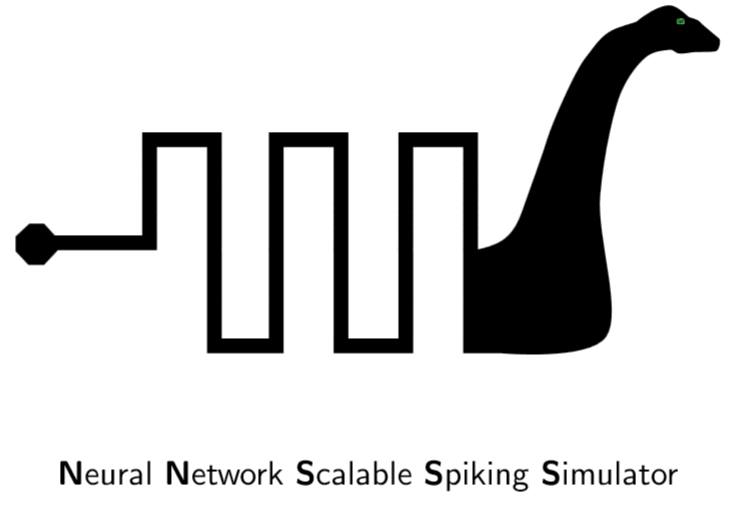
\includegraphics[scale=0.4]{image/n2s3.jpg}

\vfill
{\LARGE
\noindent
	Benjamin \textsc{Danglot}\newline
	Pierre \textsc{Falez}
}

\vfill
{
\noindent
{\LARGE Tuteur : Pierre Boulet} \hfill PJI 2015 
}

\newpage

% Table of contents

\tableofcontents

\newpage

% Introduction

\section*{Introduction}

\subsection*{Sujet} 
    Il s’agit du sujet 65 : \emph{Environnement de simulation d'un accélérateur neuromorphique}. Nous devions élaborer un langage dédié pour décrire un réseau de neurones ainsi qu’une simulation.

Mais le projet a eu d’autres besoins plus urgent, et nous avons donc développés les points importants que le simulateur avait besoin.

\subsection*{Motivations}
    Dans notre volonté de faire un doctorat, nous pensons que ce sujet était approprié pour nous apprendre des aspects de la recherche. De plus, l’utilisation de scala, et donc de son apprentissage était également un apport majeur à notre culture informatique. 
		
% Project presentation

\newpage

\section{Présentation du projet}

\subsection{Technologies}

\subsubsection{Scala} 
\begin{figure}[h!]

\includegraphics[scale=0.15,right]{image/scala.png}
\end{figure}
\paragraph
Scala est un langage de programmation multi-paradigme crée par l’Ecole polytechnique fédéral de Lausanne (EPFL). Il combine la programmation orientés objet et le fonctionnel. Le langage Scala permet également de passer à l’échelle, et le fait qu’il utilise la machine virtuelle java (JVM) permet une portabilité sur différentes plateformes et ainsi l’utilisation de cluster pour fonctionner.

\subsubsection{Akka} 
\begin{figure}[h!]

\includegraphics[scale=0.1,right]{image/akka.png}
\end{figure}
\paragraph
Akka est une bibliothèque disponible en Java et Scala qui permet d’ajouter de la concurrence et de la distribution à Scala, via un système d'acteur et de message.
        
\subsubsection{JspikeStack} 

\paragraph
JspikeStack est une application écrit en Java basé sur le modèle d'une machine de Boltzmann restreinte, qui construit et simule un réseau neuronal. Il permet notamment d’utiliser le réseau pré-appris Mnist, qui reconnaît les chiffres à partir du caméras.

\subsubsection{Memristor} 

\paragraph
Les memristors sont des composants électroniques dis passifs, il vient de la contraction de “memory” et “resistance”. Ce composant utilise sa résistance qui peut varier grâce à un courant électronique pour stocker de l’information. Le memristor a été “prédit” en 1971 par Leon Chua, mais aucun exemple physique n’a vu le jour avant 2008 par une équipe de chercheurs des laboratoires HP. Les memristors peuvent être vues comme des neurones, d’où l’implémentation d’un simulateur pour étudier le comportement de ces nouveaux composants.

\subsection{État actuel}
Notre PJI est la suite directe d’un PJI de l’année dernière, ainsi que d’un projet M2. Nous avons donc put rencontrer les étudiants qui ont démarrés le projet, et ainsi avoir une présentation de leurs travaux.

Il s’agit de l’implémentation d’un simulateur de neurone à base de “Spike”, les messages que s’échangent les neurones grâce au synapses par lesquelles ils sont reliés. Il y a plusieurs simulateur déjà existant, mais qui pose certain problème car ils (notamment BRIAN, développait en python) ont le problème de ce passage a l’échelle, et donc une limitation dans les performances de simulation. Le projet est baptisé N2S3 (Nessie) : Neural Network Scalable Spiking Simulator

Lorsque que nous avons repris le projet, ce dernier avait déjà certaines fonctionnalités partiellement ou complètement opérationnelles.

Le projet à été pensée de façon générique : il doit pouvoir s’adapter a différent modèle de réseau. Pour le moment seul le modèle QBG est implémenté (expliquer qbg => tu sais ce que c’est toah? ?). C’est pourquoi le projet est répartie dans différents packages de la façon suivante : un package core contient les classes génériques pour représenter un réseau. un package feature.io pour toutes les fonctionnalités d’entrées/sorties, un package feature.logging pour la gestion des logs et enfin un package models.qbg pour implémenter un réseau de ce type.

L’implémentation du réseau à été pensée de la manière suivante : chaque neurone et chaque synapse est représenté par un acteur. A l’époque, un synchronizer, qui est également  un agent, était en charge de récupérer tous les messages, et de les redistribuer à travers le réseau pour que la cohérence dans le temps soit bien respectée. 

Pour commencer la simulation, il suffisait de lancer des messages dans le réseau.


\subsection{Perspectives du travail réalisés}


Le fonctionnement global du simulateur fonctionne, hélas plusieurs problèmes se posent. 

La fourniture à la main d’entrées dans le simulateur n’est pas une solution convenable, de même que la création d’un réseau neuronale.

Les visualisations actuelles ne sont pas satifaisantes, et les logs ne permettent pas de bien comprendre l’évolution du réseau.

Avec un unique synchronizer pour le simulateur, le passage à l’échelle est impossible, il devient le goulot d’étranglement et ralentis toutes la progression de la simulation.

Nous avons donc travaillé sur ces points, afin de permettre à N2S3 d’évoluer.

\newpage

\section{Ajout des Entrées}

    Notre première tâche dans ce projet fût de mettre en place un système d'entrées afin de pouvoir stimuler le réseau. Celle-ci fût une bonne introduction pour nous, car elle nous a permis de prendre en main et d’aborder pas à pas le projet

    Les fichiers JAER contiennent les données produit, par exemple, par une caméra à impulsion. Ce fichier se présente sous la forme d’une liste d'évènements. Chaque évènement étant représenté par un timestamp et une source. Ainsi, notre tuteur avait déjà implémenté une classe qui lit ces fichiers à partir d’une librairie ajoutée à N2S3. 

    Pour gérer ces évènements d’entrées, nous avons créer une classe abstraite(cf InputGenerator.scala) dont l’implémentation dépendra du format de fichier d’entrée. Étant donnée que nous avions a notre disposition des fichiers JAER, et une classe de lecture, nous avons directement ajouter une classe pour ces formats de fichiers.

    Cette classe se chargera de lire, et de placer d’en une file les évènements. Dans les premières versions, la gestion des entrées était totalement “indépendante” du réseau. Tant qu’il y avait des entrées, on les envoyés au synchronizer. Mais cette méthode le surchargeait, et donc ralentissait l’évolution du réseau. A présent, le synchronizer demande des entrées lorsqu’il juge qu’il en a besoin(un seuil, ou sa file est quasiment vide). Ce qui dynamise la simulation.


\section{Création de réseau à partir de fichier XML}

Nous avons ensuite développé une classe qui permet de créer un réseau neuronale à partir d’un fichier XML.

Nous avons pris comme base, les fichiers XML utilisés par Peter O’Connor dans sa thèse. La classe permet d’initialiser le réseau, de connecté les neurones et les synapses ainsi que de leur affectés des potentiels/seuils à l’initialisation.

\section{Génération de graphes}

\paragraph
Nous avons mis en place une génération de graphe à partir des fichiers de log crée par chacun des acteurs. En effet, pour pouvoir apprécier les simulations et leurs résultats, une visualisation graphique est nécessaires.

\subsection*{Graphes d’activité des neurones}
\paragraph
A partir des logs que les neurones créent, nous pouvons générer un graphe d’activité neuronales. 

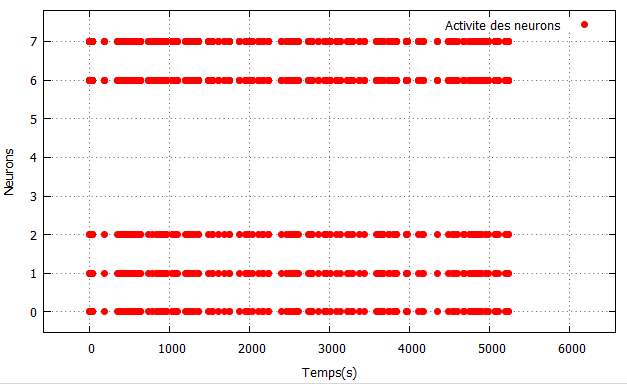
\includegraphics[scale=0.95,right]{image/neuronActivity.png}

\paragraph
Certaines options sont disponibles pour générer ce type de graphes :
\begin{itemize}
\item{Donner la liste des index des neurones que l’on souhaite observer.}
\item{Donner la liste des index des couches que l’on souhaite observer.}
\item{Donner un temps maximum.}
\end{itemize}

\subsection*{Graphes des activités des synapses}

rubarberubarberubarberubarberubarberubarberubarberubarberubarbe

\subsection{Remarques}
\paragraph
ces générations se font pour l’instant sur de petits exemples de fichiers de logs, mais il faut l’améliorer pour pouvoir visualiser sur de véritables simulations, avec des réseaux de l’ordre de millions de neurones.

\end{document}